\documentclass{beamer}
\usetheme{CambridgeUS}
\usecolortheme{seahorse}
\usefonttheme{serif}

\usepackage{lipsum}
\usepackage{graphicx,xcolor}
\usepackage{amsmath,amssymb,amsfonts}
\usepackage{realoracles}

\AtBeginSection[]{ 
    \begin{frame}{Outline} 
        \tableofcontents[currentsection] 
    \end{frame} }

\title[Oracles]{Real Numbers as Oracles}
\subtitle{Is $x$ in $a:b$}
\author{James Taylor}
\institute{ratmath.com}
\date{May 2023}

\begin{document}

\begin{frame}
\titlepage
\end{frame}


\section{Numbers}

\begin{frame}

\begin{enumerate}
\item Natural Numbers (Counting Numbers)
\item Integers (Credits and Debits)
\item Rational Numbers (Break a whole up into pieces)
\item Real Numbers (General solutions to problems)
\item Complex Numbers ($i^2 = -1$)
\end{enumerate}

\end{frame}

\subsection{Natural Numbers}

\begin{frame}{Natural Numbers}

Number as a one-to-one matching

Three fingers, three sticks, three stones, three milenia

Canonical representative?

\pause

\begin{itemize}
    \item 0 is nothing:  $\{\} = \emptyset$
    \item 1 is the container with 0:  $\{0\} = \{\emptyset\}$
    \item 2 is the container with 0 and 1:  $\{0, 1\} = \{ \emptyset,\{\emptyset\} \}$
    \item 3 is $\{0, 1, 2\}$
    \item And so on ... $n = \{0, 1, 2, \ldots, n-2, n-1\}$. 
\end{itemize}

That last step is notional and fine, but also problematical since we are defining these numbers. We build them up step by step, but there are infinitely many to do. Do we care? 

\end{frame}

\begin{frame}{Arithmetic of Natural Numbers}

The arithmetic is based on the idea of combining the items in the collection and counting. 

\pause

\begin{itemize}
\item Addition.  $2 + 3 = \{0, 1; 0, 1, 2\}$ which is 5 items. So $\simeq 5$
\item Multiplication. Repeatedly add. $2*3 =  \{0, 1, 2; 0, 1, 2\} = \{0,1; 0,1; 0,1\} \simeq 6$
\item Subtraction. Remove items, count again. Only defined if subtracting from a not smaller amount $ 3-2 = \{0, 1, 2; -0, -1\} = \{2\} \simeq 1$
\item Division. Break into groups. Want them evenly separated. $6 \div 2 = \{ (0,1), (2,3), (4,5)\} \simeq 3$
\item Exponentiation. This is repeated multiplication. $3^4 =3*3*3*3 = 81$.
\end{itemize} 

\end{frame}

\begin{frame}{Properties of Natural Number Arithmetic}

Various properties can be proved: 
\begin{itemize}
\item Commutativity: $a+b = b+a$, $a*b = b*a$
\item Associativity: $(a+b)+c = a + (b+c) = a+b+c$, $(a*b)*c=a*(b*c)=abc$ 
\item Identity: $a+0 = a$, $a*1 = a$
\item Distributive:  $a*(b+c) = (a*b) + (a*c) = ab + ac$
\end{itemize}
    
Also order of operations is defined that multiplications happen before additions unless there is parentheses involved. 

\end{frame}


\begin{frame}{Inequality of Natural Numbers}
    $a < b$ if there are more items in $b$

    This means that we can map all of the items in a representative of $a$ into one of $b$ and still have at least an item left over in $b$.

    $2 < 3$ because $\{0,1\}$ maps to $\{0, 1, 2\}$ with the $2$ leftover.
    
\end{frame}

\subsection{Integers}

\begin{frame}{Integers}

Subtracting something larger from something smaller. Wanting to define $-2$.

Inspired by assets and debts:  $(5, 7) \simeq -2$. The idea is we have $\$5$ and owe $\$7$. Our total wealth is therefore a debt of \$2. 

This is the same wealth as $(4,6)$ or $(0,2)$.

Two wealth amounts $(a,b)$ and $(c,d)$ are equivalent if $a+d = b+c$. Notice no negatives because we put the "negatives" on the other side.

For example $5+6 = 4+7$ though we are actually thinking $5-7 = 4-6$ but we added $6+7$ to both sides and got something equivalent. 

Canonical representative? 

\end{frame}

\begin{frame}{Integers}

\begin{itemize}
    \item 0 is  $(0,0)$ which is the same as $(a,a)$ for any natural number $a$.
    \item 1 is  $(1,0)$
    \item $-1$ is $(0,1)$
    \item $-2$ is $(0,2)$
    \item And so on ... $+n = (n, 0)$ and $-n = (0,n)$
\end{itemize}

The canonical representative is the one with at least one 0 in one of the slots. We can then drop the 0 and indicate whether it was in the first or second by putting a $-$ if it is in the second. 


\end{frame}

\begin{frame}{Arithmetic of Integers}

Addition comes from just adding assets and debts together. Think of two people marrying and combining their previous assets and debts into a new household. 

Negation is defined as wanting to cancel all assets and debts. So if we have $(3,4)$ then the negative is $(4,3)$ so that $(3,4) + (4,3) = (7,7) = (0,0)$

We define multiplication based on how we would combine expressions with subtraction, using the distributive property: 

$(3-6)*(5-7) = 3*5 + 7*6 - 6*5 - 21 = 57 - 51=6$ vs $-3*-2 = 6$ 


\end{frame}

\begin{frame}{Arithmetic of Integers}

\begin{itemize}
\item Addition.  $(a,b) + (c,d) = (a+c, b+d)$
\item Negation. $-(a,b) = (b, a)$
\item Subtraction. Negate and add:  $(a,b) - (c,d) = (a+d, b+c)$
\item Multiplication.  $(a,b)*(c,d) = (ac + bd, ad + bc)$
\item Division. A little tricky. Reduce to canonical representatives, do the division as if they were natural numbers, figure out the sign. 
\item Exponentiation. This is still repeated multiplication. For negative exponents, this is about reciprocating. Wait for rational numbers. 
\end{itemize} 

\end{frame}

\begin{frame}{Properties of Integer Arithmetic}

Same properties as before, but we also have the additive inverse: 

For an integer $a$, there exists $-a$ such that $a-a = 0$.

Example: $(5,7)$ has additive inverse $(7,5)$ as $(5,7)+(7,5) = (12, 12) \simeq (0,0) \simeq 0$.

Can also solve for $x$ in $x + a = b$ as $x = b-a$. Always exists for any integers $a$ and $b$.

\end{frame}

\begin{frame}{Integer Inequality}
    $(a,b) < (c,d)$ can be computed as checking $a + d < c + b$. That is we view the debt of the other as an asset of the former. 

    $(3,4) < (6,5)$ as $3+5 < 4 +6$

    In canonical form, we have $(0, 1) < (1, 0)$. 

    The more debt one has, the lower the wealth. 

    Note that because negating flips assets and debts, this means multiplying by a negative number flips the inequality. 
    
\end{frame}

\subsection{Rational Numbers}

\begin{frame}{Rational Numbers}

The rational numbers represent general division of numbers by other numbers. 

We want to understand $\frac{a}{b}$.

We have a basic unit that we are dividing into $b$ pieces. We take $a$ of those pieces.  That is what a rational number represents. $b$ is the denominator while $a$ is the numerator.

We can think of $b$ as defining a new unit and $a$ is a count in that new unit. Example:  Three dollars divided into quarters is 12 quarters. That is $3 = \frac{12}{4}$.

It is easy to see that we just add numerators if we are adding fractions with the same denominator. If we multiply a fraction by an integer, we just do that on the numerator level. 

If we think of $\frac{1}{b}$ as dividing something in $b$ pieces, then multiplying by $\frac{1}{b}$ is dividing the fraction into $b$ pieces which is multiplying the denominator by $b$. 

\end{frame}

\begin{frame}{Rational Numbers}

\begin{itemize}
    \item 0 is  $\frac{0}{1}$
    \item 1 is  $\frac{1}{1}$
    \item $-1$ is $\frac{-1}{1}$
    \item $\frac{3}{6}$ is $\frac{1}{2}$
\end{itemize}

The canonical representative is the one with no common factors in the denominator and numerator. For $0$, we choose the denominator of $1$ for definiteness. 


\end{frame}

\begin{frame}{Arithmetic of  Rational Numbers}

For addition, we need to have common denominators. Then we just add the numerators. 

For multiplication, we just multiply top and bottom. 

If we were to add the top and bottom, we get mediants which are useful, but not the addition that we are looking for. 

$\frac{4}{3} + \frac{5}{6} = \frac{8}{6} + \frac{5}{6} = \frac{13}{6}$ 

Also the same as blindly multiplying the denominators to get the common denominator:  $\frac{24 + 15}{18} = \frac{39}{18}$.

$\frac{4}{3} * \frac{5}{6} = \frac{20}{18} = \frac{10}{9}$.

\end{frame}

\begin{frame}{Arithmetic of  Rational Numbers}


\begin{itemize}
\item Addition.  $(a,b) + (c,d) =  (ad+ bc, bd)$
\item Negation. $-(a,b) = (-a, b)$
\item Subtraction. Negate and add:  $(a,b) - (c,d) = (ad -bc, bd)$
\item Multiplication.  $(a,b)*(c,d) = (ac, bd)$
\item Reciprocation. $(a,b)^{-1} = (b, a)$
\item Division. $(a,b) \div (c,d) = (ad, bc)$
\item Exponentiation. This is still repeated multiplication. For exponents with denominators, we need $n$-th roots which require real numbers. 
\end{itemize} 

\end{frame}

\begin{frame}{Properties of Rational Numbers}

Same properties as before, but we also have the multiplicative inverse: 

For a rational number $q$, there exists $\frac{1}{q} = q^{-1}$ such that $q*\frac{1}{q} = 1$. In particular, $\frac{a}{b} * \frac{b}{a} = \frac{ab}{ab} \simeq 1$

Example: $\frac{2}{3}$ has multiplicative inverse $\frac{3}{2}$ as $\frac{2}{3} * \frac{3}{2} = \frac{6}{6} \simeq 1$.

Can also solve for $x$ in $a*x = b$ as $x = b/a$. Always exists for any rational numbers $a$ and $b$ as long as $a \neq 0$.

\end{frame}

\begin{frame}{Inequality of Rational Numbers}
    Compare numerators when they have common denominators. 

    $\frac{a}{b} < \frac{c}{d}$ when $\frac{ad}{bd} < \frac{bc}{bd}$ which is the same as $ad < bc$ or $bc-ad > 0$.

    $\frac{1}{3} < \frac{3}{4}$ as $\frac{4}{12}< \frac{9}{12}$ also $4 < 9$ or $9-4 = 5 > 0$.

\end{frame}


\subsection{Real Numbers}

\begin{frame}{Real Numbers}
    We will elaborate on these at length. But for now, they solve equations such as $x^2 = 2$ leading to $\sqrt{2} = 1.41421356237...$

    They also provide us with $\mathrm{e} = \lim_{n \to \infty} (1+\frac{1}{n})^n  = 2.718281828...$

    And $\pi$ which gives us the area of a circle of radius $r$ as $\pi r^2$; the circumference is $2 \pi r$. $\pi = 3.14159265....$

    What are those $\ldots$ saying?  What are these numbers?  
    
\end{frame}

\subsection{Complex Numbers}

\begin{frame}{Complex Numbers}

Trying to solve $x^2 + 1 = 0$. Doesn't make sense since $x^2$ is never negative for real numbers and 1 is certainly not negative. So how can this be solved? 

Introduce a new thing, $\sqrt{-1}$ which has the property that $\sqrt{2}^2 = -1$. 

The usual notation is $\mathrm{i}$ for imaginary (also $\mathrm{j}$ is used by engineers).

We then define the complex numbers as $a + b \mathrm{i}$ and define the arithmetic as we usually would, but with using $\mathrm{i}^2 = -1$. 

Also, $\frac{1}{\mathrm{i}} = - \mathrm{i}$ which is neat and weird. 

\end{frame}

\begin{frame}{Complex numbers}

We can view these as ordered tuples. 

\begin{itemize}
    \item 0 is  $(0,0)$
    \item 1 is  $(1,0)$
    \item $-1$ is $(-1,0)$
    \item $\mathrm{i}$ is $(0,1)$
    \item $-\mathrm{i}$ is $(0, -1)$
    \item $1+\mathrm{i}$ is $(1,1)$
    \item $27.4 -57 \mathrm{i}$ would be $(27.4, -57)$
\end{itemize}

There is only one version of this number. This makes the number system 2 dimensional. The others had an aspect of two dimensionality that would get collapsed into one dimension. Here we have two dimensions. 


\end{frame}

\begin{frame}{Arithmetic of Complex Numbers}

We define arithmetic based on how we would combine expressions with using the distributive property: 

$ (3 + 2\mathrm{i})*(5 + 7\mathrm{i}) 
 =  15 +21 \mathrm{i} + 10 \mathrm{i} + 14 \mathrm{i}^2 $

Using $\mathrm{i}^2 = -1$, we have  $ 15 - 14 + (21 +10) \mathrm{i} = 1 + 31\mathrm{i} $
 
\end{frame}

\begin{frame}{Arithmetic of Complex Numbers}

$(a,b)$ is the same as $a + b \mathrm{i}$

\begin{itemize}
\item Addition.  $(a,b) + (c,d) = (a+c, b+d)$
\item Negation. $-(a,b) = (-a, -b)$
\item Subtraction. Negate and add:  $(a,b) - (c,d) = (a-c, b-d)$
\item Multiplication.  $(a,b)*(c,d) = (ac - bd, ad + bc)$
\item Reciprocation. $\frac{1}{(a,b)} = \frac{1}{a+b \mathrm{i}} \frac{a-b\mathrm{i}}{a - b \mathrm{i}} =  \frac{a - b \mathrm{i}}{a^2 + b^2}$.
\item Division. Reciprocate and multiply. 
\item Exponentiation. For positive exponents, this is still repeated multiplication. $n$ distinct solutions to $x^n = 1$. For complex exponents, this gets complicated. 
\end{itemize} 

\end{frame}

\begin{frame}{Properties of Complex Arithmetic}

All the properties as before, including additive and multiplicative inverses. 

If we are complexifying the real numbers, then all polynomials with complex coefficients have solutions.

This is the Fundamental Theorem of Algebra. It has many proofs, none of which are simple or direct.  

\end{frame}

\begin{frame}{Inequality of Complex Numbers}
    There is no ordering of the complex numbers that respects addition. 

    This is 2 dimensions and ordering is basically one dimensional. 

    Would $i$ be positive or negative?  Squaring of a number with inequality makes it positive generally. But not here. 

    Sorry!
\end{frame}


\section{Real Numbers as Oracles}

\begin{frame}{Something Different}

The counting numbers are our foundations and they are different from what follows. Integers, rational numbers, and complex numbers are similar as being ordered pairs and can even be introduced in any order. They are necessary and open up many vistas, but their definitions are shrugs. 

Real numbers, however, are very different. They are an entirely different kind of thing. We start with a decimal viewpoint and see what is wrong with it. 

\end{frame}

\subsection{Decimals}

\begin{frame}{Rational Decimals}
    Decimals are rational numbers whose denominators are powers of 10: 10, 100, 1000, 10000, ...

    The number $0.34$ is a compact way of writing $\frac{34}{100}$. 

    For some rational numbers, we can convert directly to decimal:  $\frac{3}{4} = \frac{3*25}{4*25} = \frac{75}{100}$.

    For others, we can only approximate with a finite decimal: $\frac{1}{3} =  \frac{333}{999} = \frac{33,333}{99,9999}$. If we squint and round the 9's expressions to the nearest power of 10, we get $0.333$ and $0.33 333$ for those fractions. We can see that $0.33333333\ldots = 0.\bar{3}$.

    All rational numbers have periodic decimal expansions; all periodic decimal expansions are rational numbers. Most computations require long division. 

    Arithmetic is just that of rational numbers:  $0.12+0.347= \frac{12}{100}+\frac{347}{1000} = \frac{120+347}{1000} = 0.467  $  and $0.23*0.5 = \frac{23}{100}*\frac{5}{10} = \frac{115}{1000} = 0.115$.
    
\end{frame}

\begin{frame}{Any Old Decimals}

    From the nice predictable decimals, a natural question is, what about the others? What if we had a decimal that kept changing, going on forever? 

    The square root of 2 is not rational and so it has to be nonperiodic if we write down its deimals. 

    In fact, WolframAlpha tells us

    $\sqrt{2} = 1.414213562373095048801688724209698078569671875376948073\ldots$

    That is why more numbers than we need, but why short of what is required to say what it is. 
    
\end{frame}

\begin{frame}{Issues of Infinity}

    Infinity is difficult. If we view real numbers as decimals, we are stating that it is an infinite string of digits. This has some issues: 

    \begin{itemize}
        \item We can never express it. 
        \item Most random strings of infinite digits will be the Library of Babel. Encode the digits into an alphabet and every possible history, every possible book, every textual representation will eventually appear. Infinity is big. This is called being normal. 
        \item Arithmetic is impossible to do accurately. What are the tools we have to deal with this? 
    \end{itemize}

    As an example, $\frac{1}{9} = 0.\bar{1}$. Consider $\frac{1}{9}*\frac{1}{9} = \frac{1}{81} = 0.\overline{012345679}$ but do this multiplication out as a decimal. We end up adding more and more 1's as we go out to the right and this pattern mysteriously appears. 
    
\end{frame}

\begin{frame}{Loss of Precision}

    A crucial issue is that if approximate infinite decimals and then do arithmetic, the precision generally gets worse. 

    For example, approximating $\sqrt{2}^2$ as $1.41*1.41 = 1.9881$. If we viewed our approximation as truncation, then 1.41 represents the interval $1.41:1.42$.  Applying that to $1.9881$, we would present it as $1.98$ representing $1.98:1.99$. Even if we round up first, we get $1.99:2.0$ which just barely includes $2$.

    With more arithmetic, particularly multiplying by larger numbers, the interval of uncertainty expands. 

    There are rules of thumbs that get put under ``significant figures'' to try to address this, but what we really need is to use intervals.  For example, if we have $1.41:\sqrt{2}:1.42$ then $1.41^2 : (\sqrt{2})^2 : 1.42^2 = 1.9881 : (\sqrt{2})^2 : 2.0164$ which gives a precise interval containing our imprecision. 

    
\end{frame}

\subsection{Pathways}

\begin{frame}{Some Possibilities}
    \begin{itemize}
        \item Decimals. Take the infinite string of decimals as defining real numbers. We have seen some of the issues. 
        \item Cauchy Sequences. Define a real number as a sequence of numbers that are trapped in ever smaller intervals. Not unique, notice the shadow of the intervals.   
        \item Dedekind Cuts. Truncation of decimals gives us numbers always less than or target, but they creep up to it. So take the number as the set of all numbers less than it. Not very helpful but common.
        \item Family of Overlapping, Notionally Shrinking Intervals (fonsis). A collection of intervals that have as small an interval as we want in them, but they all overlap. The core of the overlap is the real number. 
    \end{itemize}

Fonsis are excellent tools for dealing with real numbers, but they are not unique. They can be extended up to the maximal fonsi which are the Yes intervals of the oracles...
    
\end{frame}

\begin{frame}{Criteria}
    

What are some good properties of a definition of real numbers? 

\begin{itemize}
    \item Uniqueness. Given a target real number, there should be only one version of that in the real number system.
    \item Reactive. Real numbers generally have an infinite flavor to them. Do not pretend we can write infinity; rather present a method of answering queries. 
    \item Rational-friendly. Rationals easy to see, easy to work with. 
    \item Supportive. Numbers should conform to how numbers are used in science, applied mathematics, and numerical analysis. 
    \item Delayed Computability. The definition should not require computing it out, but should facilitate it. 
    \item Arithmeticizable. Arithmetic should be doable with measurable progress. 
    \item Resolvability. Some real numbers are inherently unknowable; does the definition give tools to handle that? 
\end{itemize}

\end{frame}

\subsection{Oracles}

\begin{frame}{Oracle Rules}

    An oracle is a rule that, given to rational numbers, say Yes or No. It says Yes if the real number ought to be inclusively between the two rational numbers and No otherwise. The two rational numbers can be equal (singleton). 

    We write $a:b$ to represent the inclusive interval between $a$ and $b$. There is no implied ordering. If $a \leq b$, we can write $a \lte b$ to denote that. 

    There are five properties that a rule $R$ must satisfy to be a real number oracle. 

\end{frame}

\begin{frame}{Oracle Properties}

\begin{enumerate}
    \item Consistency. If an interval contains a Yes interval, then it is a Yes interval. This maintains the illusion of the real number being in the Yes intervals and also leads to this being a unique representative of a real number. 
    \item Existence. There should be a Yes interval, i.e., there is something there. 
    \item Closed. If a rational number is in every Yes interval, then its singleton should also be a Yes interval. 
    \item Rooted. There is at most one Yes singleton.  This helps ensure that the oracle is narrowed in on a single number. 
    \item Interval Separation. This is the key property. For a given Yes interval, a point $c$ inside that interval creates two subintervals in addition to its own singleton. The requirement is that exactly one of those intervals is Yes unless $c:c$ is a Yes singleton, in which case all three are Yes since $c$ is in all three.  
\end{enumerate}

\end{frame}

\begin{frame}{Rationals as Oracles}
    If we have a rational $\frac{p}{q}$, what is the oracle that represents it? 

    Easy: An interval is a Yes interval if $\frac{p}{q}$ is contained in it. 

    This includes the singleton $\frac{p}{q}:\frac{p}{q}$ which is the canonical representative of the rational oracle. 

    We may also call these singleton oracles or rooted oracles. 
\end{frame}

\begin{frame}{Aside: Pythagorean Theorem}
    For a right triangle with side lengths $a$, $b$, and hypotenuse $c$ we have $a^2 + b^2 = c^2$.

    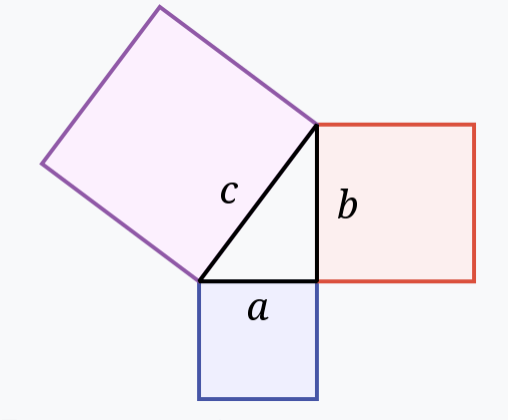
\includegraphics[width=3in]{Images/pythagoras.png}

\end{frame}

\begin{frame}{Aside: Pythagorean Theorem}

    Proof:  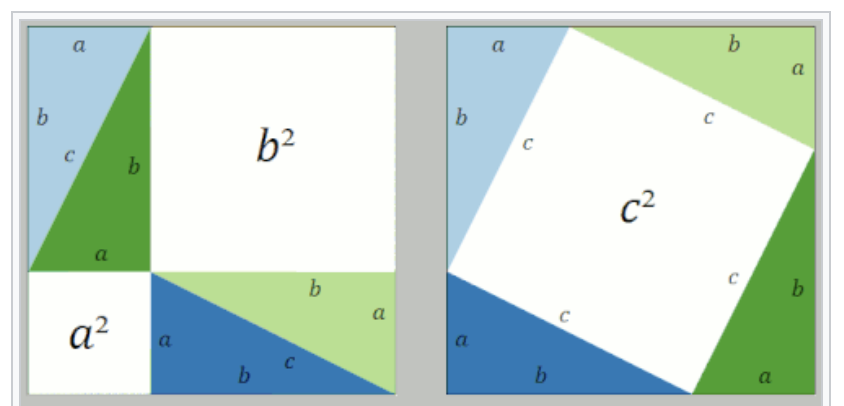
\includegraphics[width=\textwidth]{Images/pythagoras-proof.png}

    From Wikipedia: \url{https://en.wikipedia.org/wiki/Pythagorean_theorem}
    
\end{frame}

\begin{frame}{Diagonal of the Unit Square}
    The unit square has side lengths 1. Draw in the diagonal. We get two right triangles. What is the length of the hypotenuse? 

    $c^2 = 1^2 + 1^2 = 2$  So we need a number $c$ such that $c*c = 2$. This is the square root of 2 or $\sqrt{2}$.

    What is the square root of 2?  If we look at $(\frac{p}{q})^2 = 2$, then $p^2 = 2q^2$ and $p$ is even, but this then implies two 2's on the left and so $q$ must be even implying three 2's on the right which makes $p$ have another factor of 2 and so we keep repeating and conclude there are infinitely many 2's on both sides. So the square root of 2 is not rational. 

    But we can measure it.
    
\end{frame}

\begin{frame}{Geometrically Computing $\sqrt{2}$}
    Consider a $3-4-5$ right triangle. Notice $3^2 + 4^2 = 5^2$. This exists. 

    This generates a $1 - 4/3 - 5/3$ right triangle and a $3/4 -1 - 5/4$ right triangle. 

    So  $\frac{5}{4} : \sqrt{2} : \frac{5}{3}$

    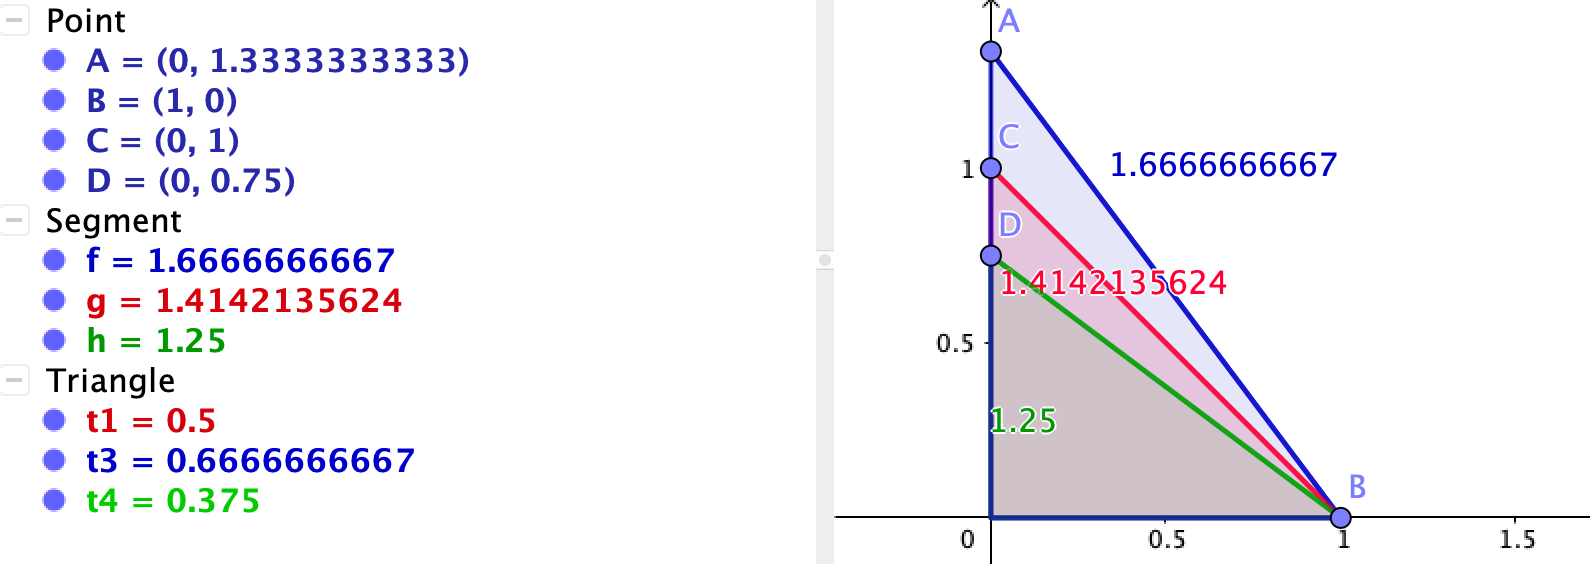
\includegraphics[width=\textwidth]{Images/pythagoras-sqrt-2.png}

    GeoGebra: \url{https://www.geogebra.org/m/mxnqaqpx}
    
\end{frame}


\begin{frame}{Root 2 Intervals}
    A better way to compute a square root.

    If we guess $x$ for the answer, then $\frac{2}{x}$ is its partner and we have $x : \sqrt{2} : \frac{2}{x}$.  

    Example: $x=\frac{3}{2}$ has partner $\frac{2}{3/2} = \frac{4}{3}$. So $\frac{4}{3} : \sqrt{2} \frac{3}{2}$.

    To get a next guess, pick anywhere in the interval and repeat. The middle is reasonable: 

    $\frac{1}{2} (\frac{3}{2} + \frac{4}{3}) =  \frac{9 + 8}{2*6} = \frac{17}{12}$. Its partner is $\frac{24}{17}$.  

    In decimals, we have $1.411 : \sqrt{2} : 1.4167$. 

    Next:  $\frac{1}{2} (\frac{17}{12} + \frac{24}{17} ) =  \frac{577}{408} \approx 1.414211438$

    Partner:  $\frac{2}{577/408} = \frac{816}{577} = 1.14211438$. The square root of 2 is in between these two numbers. 
    
\end{frame}

\begin{frame}{$n$-th Roots}

    Generically,  if we are trying to solve $x^n = q$, with guess $x$, then $\frac{q}{x^{n-1}}$ is its partner. 

    Find the cube root of 17. Since $2^3 = 8 : 17 : 27=3^3$ we could guess $\frac{5}{2}$. Then $\frac{17}{ (5/2)^2 }  = \frac{68}{25} \approx 2.72$  So $2.5:\sqrt[3]{17}:2.72$.

    Next guess is a weighted average, weighting the guess: $\frac{1}{n} ((n-1) x + \frac{q}{x^{n-1}})$

    Here that is $\frac{1}{3} ( 5 + \frac{68}{25}) = \frac{193}{75} \approx 2.573$

    Partner is $\frac{95625}{37249} \approx 2.567$

    The cube root of $17$ is about $2.57128$. 
\end{frame}


\begin{frame}{Compound Interest}
    Interest at nominal $100\%$ rate, compounded over a year, say daily, is $(1+\frac{1}{365})^{365}$ is about $2.7145$.

    What is that number?  That is approximately $\mathrm{e}$. 

    Math people would write $\mathrm{e} = \lim_{n \to \infty} (1+\frac{1}{n})^n$

    What does that mean? 

    Clarity comes from proving (not here) that $(1+\frac{1}{n})^n : \mathrm{e} : (1+\frac{1}{n+1})^{n+1}$
    
\end{frame}

\begin{frame}{Large $n$  for e}

\begin{itemize}
    \item $n=1$  $(1+1)^1 = 2 : (1+1)^2 = 4$
    \item $n=2$  $(1+1/2)^2 = \frac{9}{4} : (1+1/2)^3 = \frac{27}{8} $
    \item $n=100$  $(1+ 1/100)^{100} \approx 2.7048 : (1+ 1/100)^{101} \approx 2.7319$  
    \item $n$ is a million  $2.7182804:2.7182832$

\end{itemize}

    Slow convergence, but we do get to $e\approx 2.71828318$.

    Recommend using WolframAlpha. 
    
    The summation $s_n = \sum_{k=0}^{n} \frac{1}{k!}$ works way better: $s_5 = 1 + 1 + \frac{1}{2} + \frac{1}{6} + \frac{1}{24} + \frac{1}{120} = \frac{240 + 60 + 20 + 5}{120} = \frac{325}{120} \approx 2.708$

    Summing up to 20, we get $s_{20} \approx 2.7182818285$. 

    It can be shown that  $s_n : \mathrm{e} : s_n + \frac{1}{n!n}$  For $n=20$, we have $20!20 \approx 4\times 10^{19}$. Thus the $s_n$ is accurate to within 18 decimal places or so. 
    
    
\end{frame}


\begin{frame}{Area and Circumference of the Unit Circle}
    
    The area of the circle with radius $r$ is $\pi r^2$ and the circumference is $2 \pi r$.

    What is $\pi$?  There are many, many ways to calculate it. 

    The simplest, but pretty slow method, is to put something inside the unit circle (inscribe) and something outside the unit circle (circumscribe) where those somethings are things we can actually compute out. 

    We can use regular polygons, such as a square or a hexagon. 

    By having an outer and inner, we get an interval that traps $\pi$. As $n$ gets larger, that interval shrinks. 

    We can use area or circumference. 
    
\end{frame}


\begin{frame}

    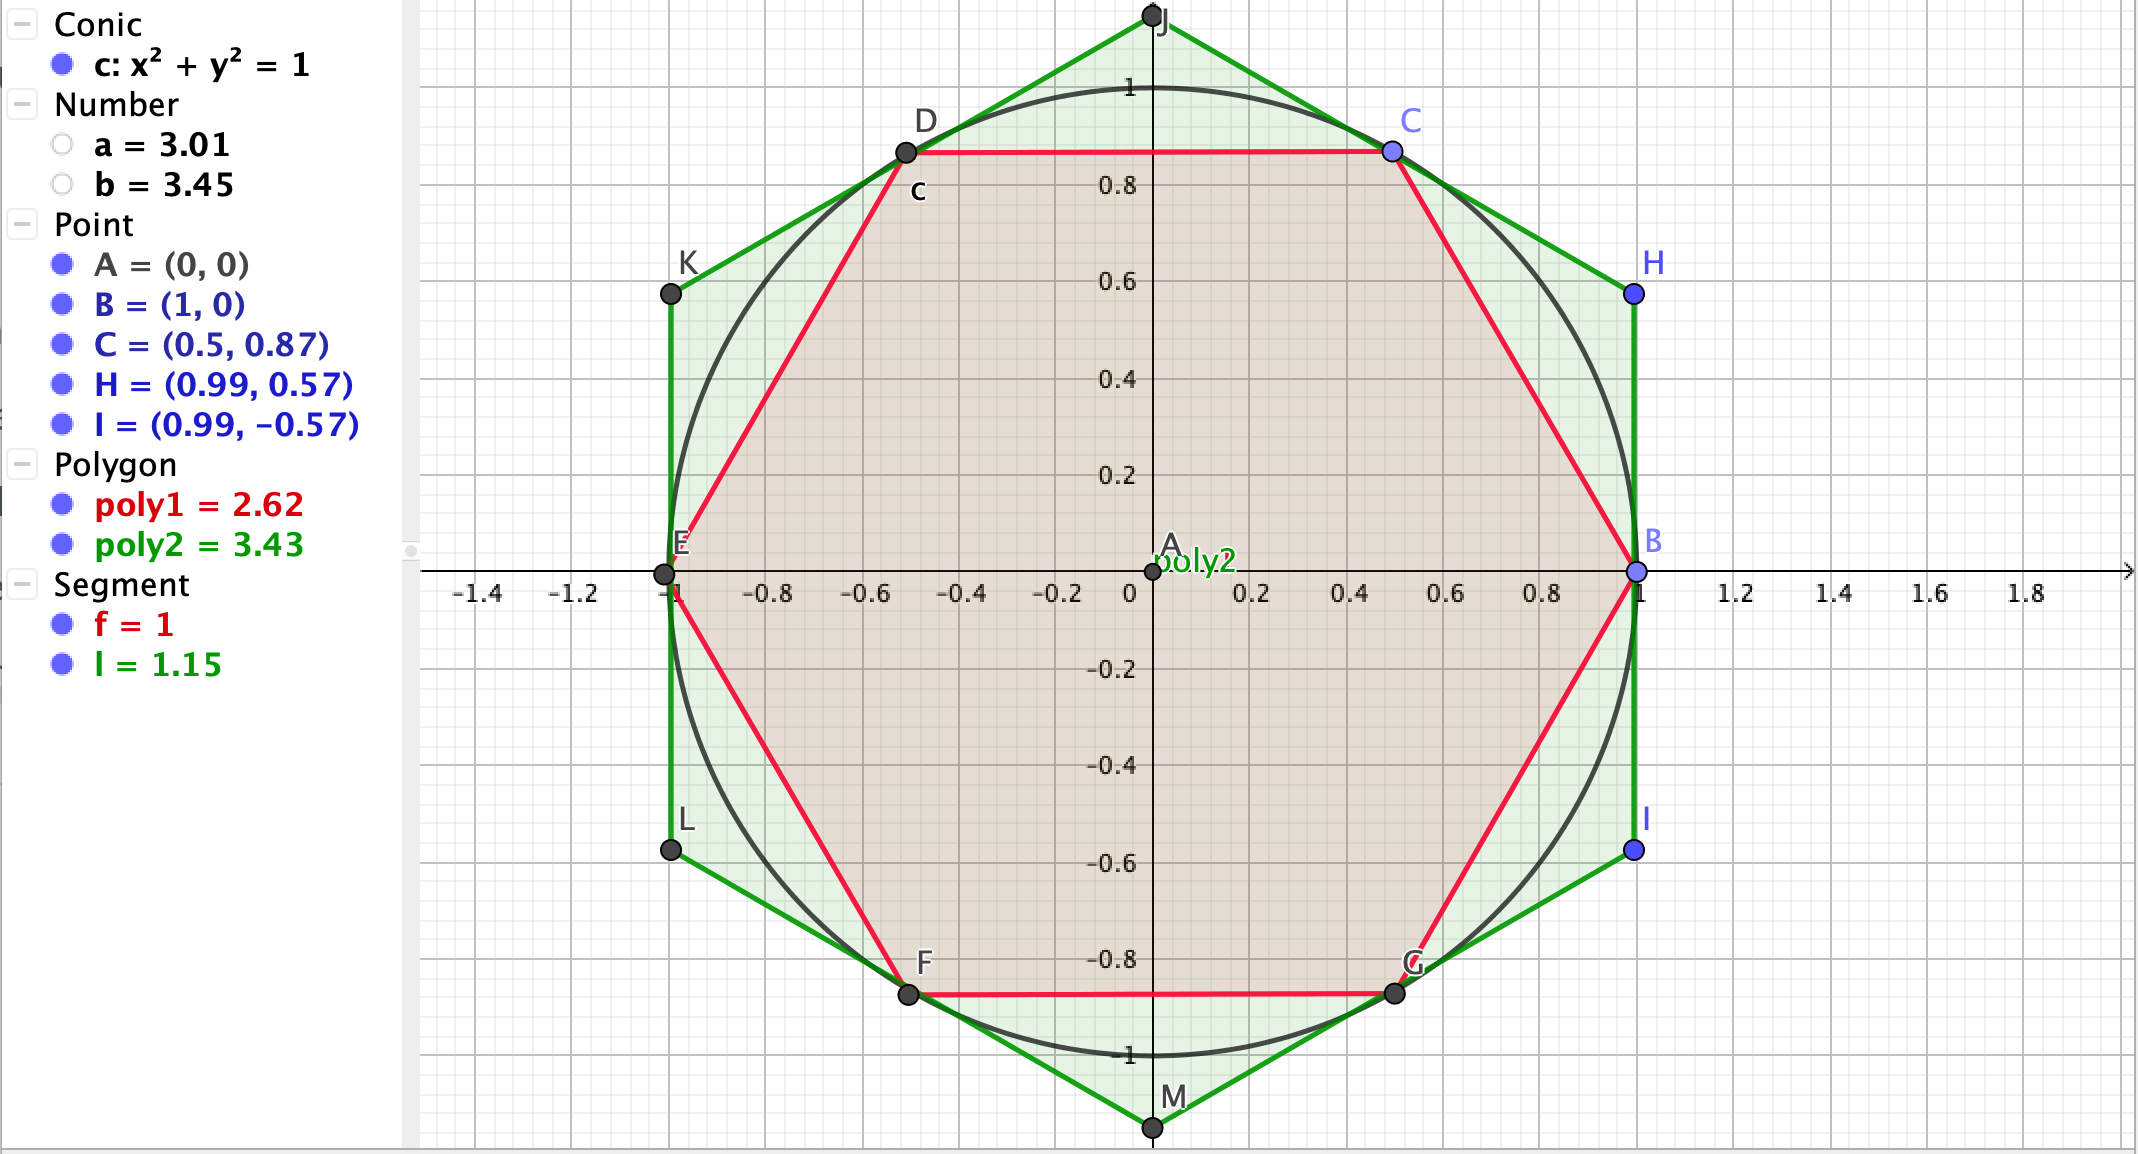
\includegraphics[width=\textwidth]{Images/hexagon-circle.png}

  GeoGebra construction:  \url{https://www.geogebra.org/m/wwcp4bbh}
  
  a and b are half the perimeters, poly1 and poly2 are the areas.
\end{frame}


\begin{frame}

   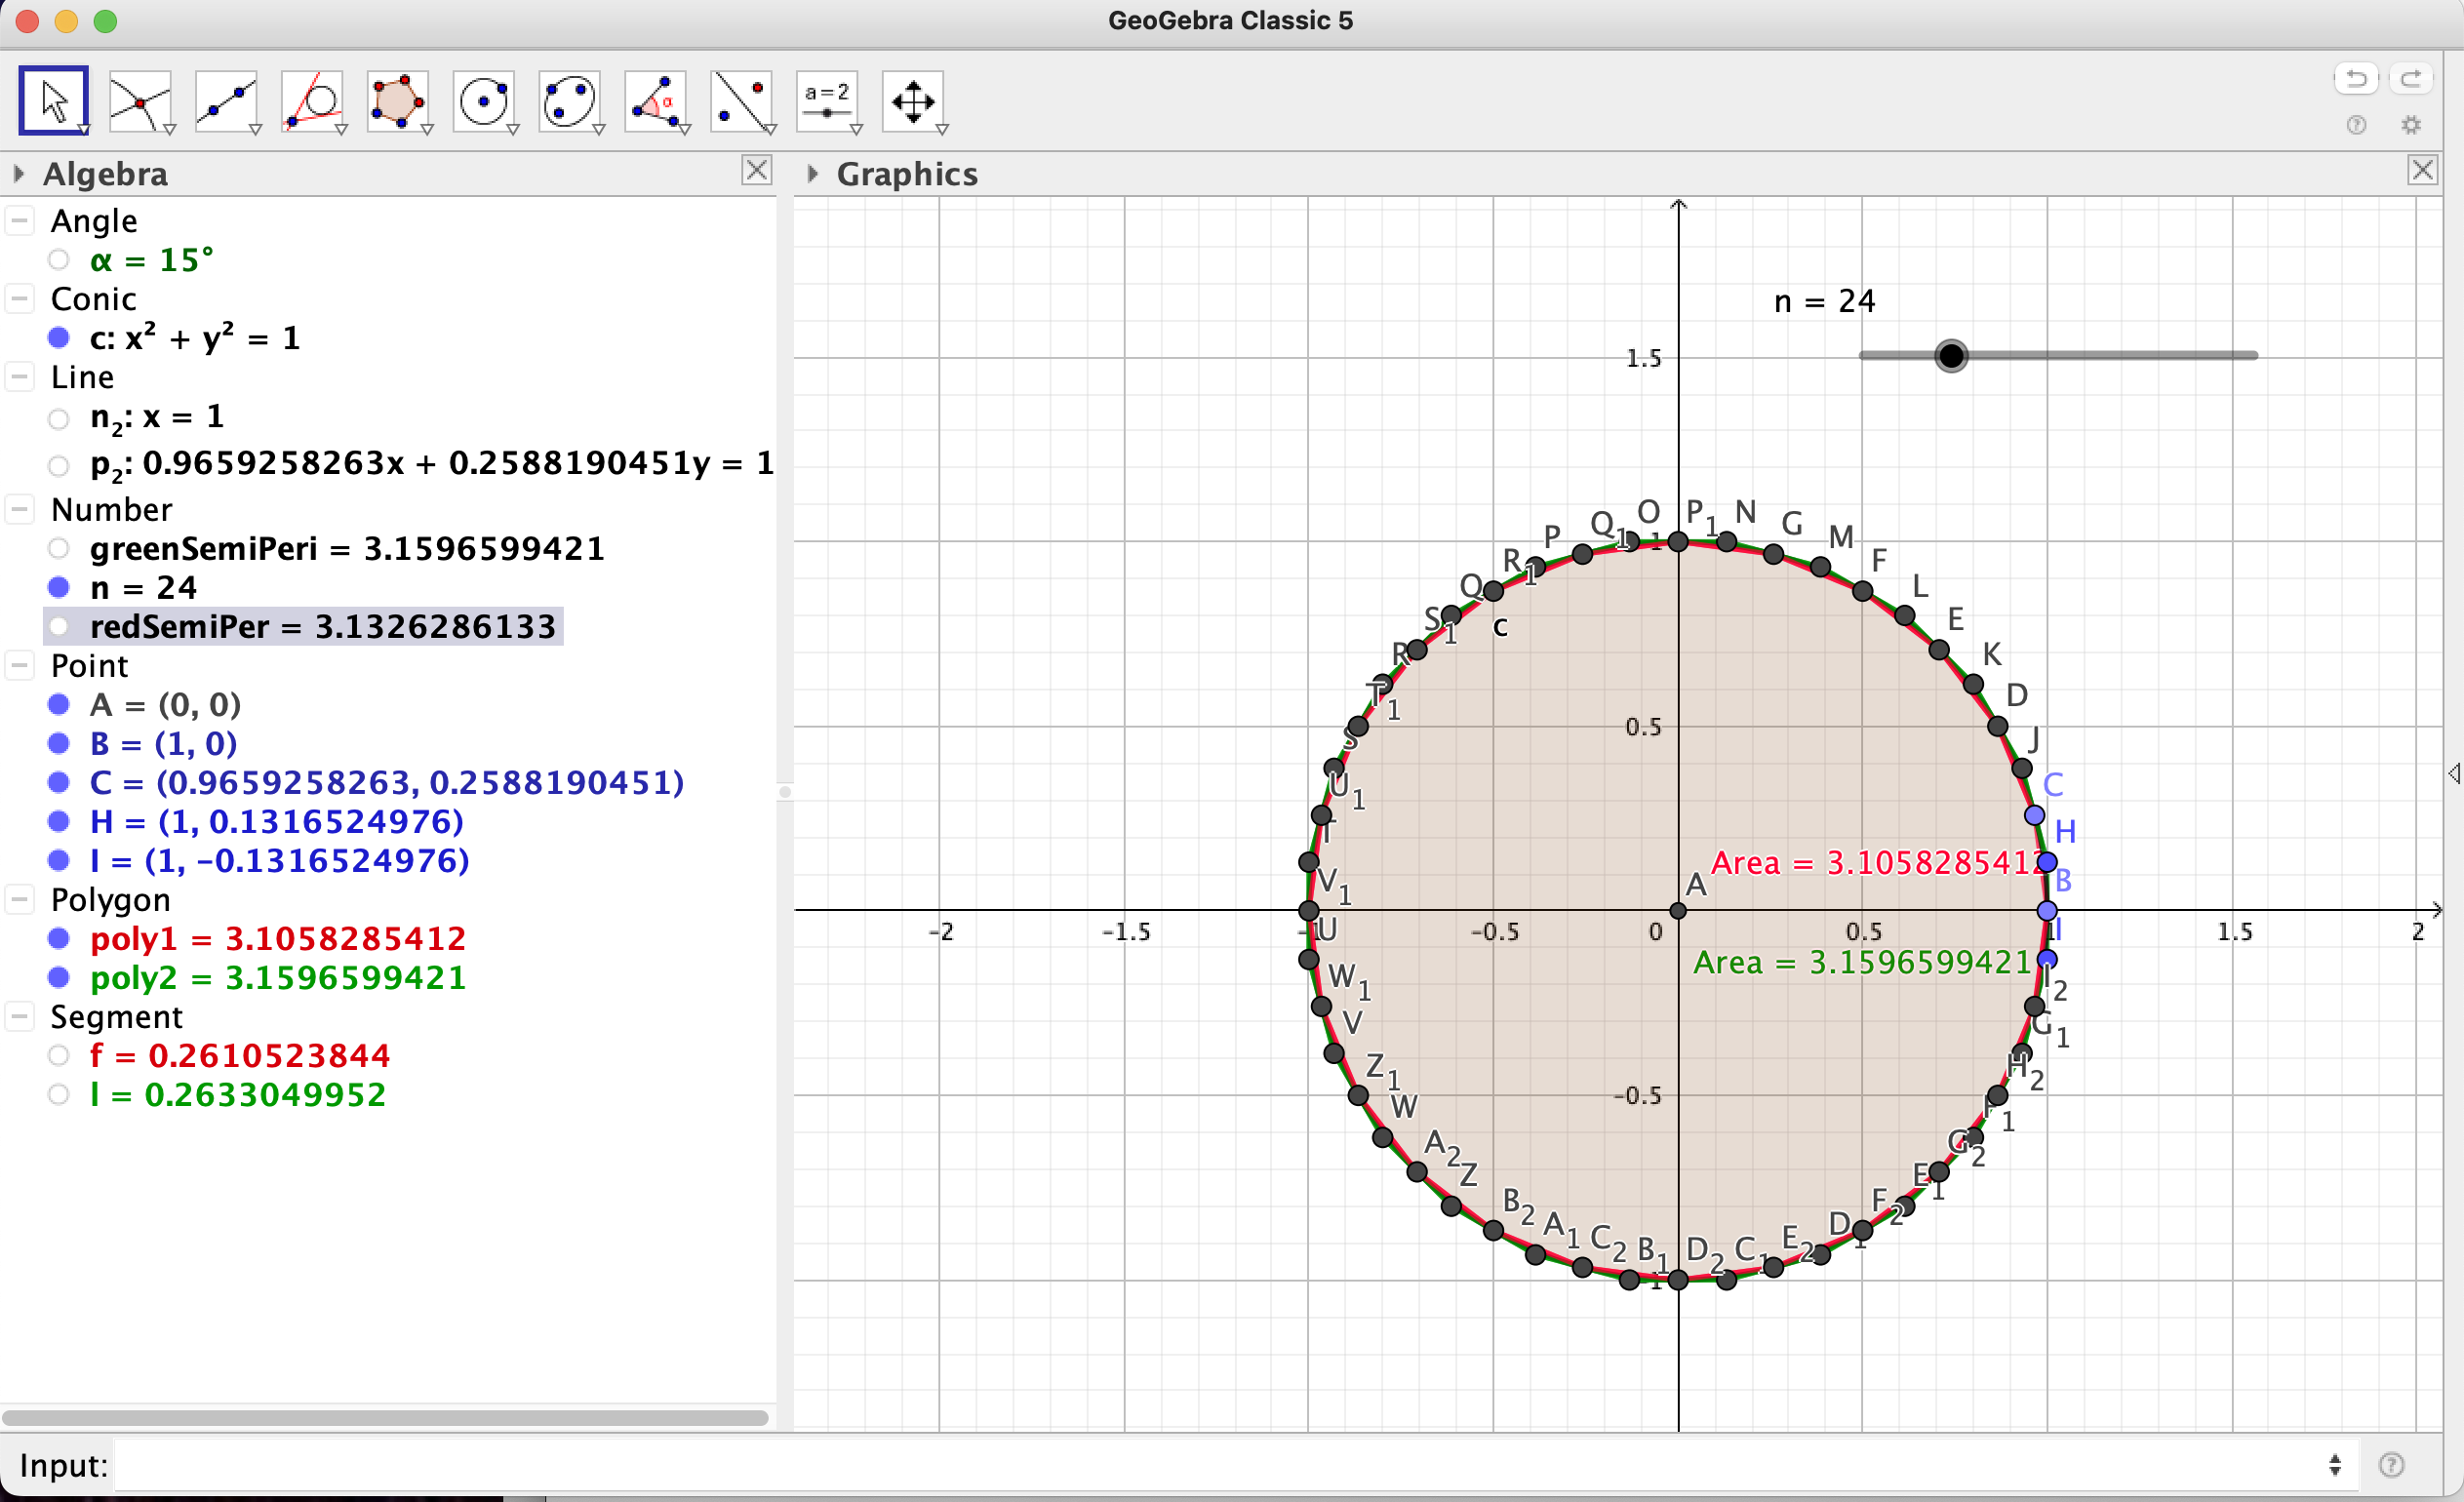
\includegraphics[width=\textwidth]{Images/flexible-hexagon-circle-24.png}

  GeoGebra construction:  \url{https://www.geogebra.org/m/fcjmp9g6}
  \begin{tiny}
  Construction: Use 360/n for angle to put C at $(\cos(\alpha), \sin(\alpha))$, draw tangents through B and C to get H as intersection of tangents,  get I as reflection of H. Regular polygon defined by number of sides and one segment. 
  
  \end{tiny}
\end{frame}


\subsection{Completions}

\begin{frame}{Limits}

Claim: Any sequence of numbers such that the tail can be contained in any arbitrarily small interval does have a limit. 

Example: The geometric sums $s_n = \sum_{k=0}^n (\frac{1}{2})^n$. For any $m \geq n$, we have\footnote{$(1-\frac{1}{2} ) s_n = s_n - \frac{s_n}{2} = 1 + \frac{1}{2} + \cdots \frac{1}{2^n} - \frac{1}{2} - \cdots -\frac{1}{2^n} - \frac{1}{2^{n+1} } = 1 - \frac{1}{2^{n+1}}$ } $\frac{1 - (\frac{1}{2})^{n+1}}{1 - \frac{1}{2}}= 2 (1 - (\frac{1}{2})^{n+1}):s(n):2$. Since the only number common to all of them is $2$, we have $\sum_{k=0}^{\infty} (\frac{1}{2})^n = 2$

The limit oracle says exactly Yes to any interval that contains the tail of the sequence. 


    
\end{frame}

\begin{frame}{Least Upper Bounds}

Claim:  Any set that is bounded above has a least upper bound. 

Example:  The set of numbers whose square is less than 2. 

The Least Upper Bound Oracle:  The least upper bound oracle says Yes to an interval if its lower endpoint is less than or equal to all the upper bounds of the set while its upper endpoint should be greater than or equal to all the elements of the set. 
    
\end{frame}

\begin{frame}{Intermediate Value Theorem}

Claim: If a function $f$ is nice and going in one direction in a given interval, say $I$, and it is negative at one endpoint of $I$, but positive at the other endpoint, then there is an input at which it is $0$.

Example: $x^2 -2$ on $0:\infty$,  $\ln(x) = 1$, $\sin(x) = 0$ on $3:4$

The Solution Oracle:  An interval $a:b$ contained in $I$ is a Yes interval if $( f(a) - y)(f(b) - y) < 0$. Intervals not contained in $I$ are decided on by Consistency. 
    
\end{frame}


\section{Arithmetic}

\begin{frame}{Oracle Arithmetic}
    A core part of the difficult of real numbers is dealing with arithmetic. 

    We approach it by first doing arithmetic with intervals. 

    Then we argue that since we can take as narrow intervals as we like, we can make those arithmetic intervals as small as we like. 

    This gives a real number arithmetic with precision about its imprecision. 
\end{frame}

\begin{frame}{Interval Arithmetic}

    How do we combine intervals?  
    Let $a \leq b$ and $c \leq d$, all of them being rational numbers. Then we define:
\begin{enumerate}
    \item Addition. $a\lte b \oplus c\lte d = (a+c)\lte (b+d)$
    \item Negation. $\ominus\ a\lte b = -b\lte -a$
    \item Subtraction. $a\lte b \ominus c\lte d = a\lte b \oplus (-d\lte -c) = a-d\lte b-c$
    \item Multiplication. $a\lte b \otimes c\lte d = \min(ac, ad, bc, bd)\lte  \max(ac,ad,bc,bd)$. For $0<a<b$ and $0<c<d$, this is equivalent to $a\lte b \otimes c\lte d = ac\lte bd$. 
    \item Reciprocity. $1 \oslash (a\lte b) = \frac{1}{b}\lte \frac{1}{a}$ as long as $a\lte b$ does not contain 0. If 0 is contained in $a \lt b$, then the reciprocal is undefined as it actually generates the split interval of $-\infty\lte \frac{1}{a}$ and $\frac{1}{b}\lte \infty$.
\end{enumerate}



\end{frame}

\begin{frame}{Interval Arithmetic Properties}
    Associativity, Commutativity, and Identities carry over, but there are no inverses as interval arithmetic never shrinks an interval. The only exceptions are the singletons. 
    
    The distributivity property becomes a containment statement:   $I = a:b\otimes(c:d \oplus e:f)$ is contained in $J = (a:b \otimes c:d) \oplus (a:b \otimes e:f)$. 
    
\end{frame}

\begin{frame}{Interval Arithmetic Examples}


    \begin{enumerate}
        \item  $3:4 \oplus \frac{2}{3}:\frac{3}{4} = 3 \frac{2}{3} : 4 \frac{3}{4}$.
        \item  $3:4 \otimes \frac{2}{3}:\frac{3}{4} = 2 : 3$
        \item  $\ominus 3:4 = -4:-3$
        \item  $1\oslash 3:4 = \frac{1}{4} \lte \frac{1}{3}$.
        \item  $3:4 \otimes -2:3$  Compute all the endpoints:  $-6, -8, 9, 12$ to get $-8:12$. A length of 1 and 5 led to a length of 20. 
    \end{enumerate}

\end{frame}

\begin{frame}{Narrowing}
    To go from interval arithmetic to oracle arithmetic, we need to observe that if we do arithmetic with interval $I$ and $J$ that are contained in intervals $K$ and $L$,  then the result of combining $I$ and $J$ is contained in $K$ and $L$. Not only that, but we can figure out how small $I$ and $J$ need to be in order for the result to be smaller than a given bound. 

    That is, by taking narrower and narrower intervals, we can narrow in on the result we are trying to compute. 

    So oracle arithmetic combination leads to fonsis and fonsis can always be made into oracles (filling in the missing intervals by consistency and closed). 

    When we do this, we get inverses and the distributive property as well as all the other properties. 
    
\end{frame}

\begin{frame}{$\frac{\mathrm{e} - \sqrt{2}}{\pi}$}

    We want to compute the oracle of this. This means, we need to answer a question such as is $Q = \frac{41}{100}: \frac{42}{100}$ a Yes interval?

\begin{enumerate}
\item $e$-Yes interval $A  = \frac{106}{39} \lte \frac{87}{32}$,
\item $\sqrt{2}$-Yes interval $B = \frac{41}{29} \lte \frac{17}{12}$, and
\item $\pi$-Yes interval of $C= \frac{333}{106} \lte \frac{22}{7}$.
\end{enumerate}
The interval operations are then as follows:
\begin{enumerate}
\item Subtraction is $A\ominus B = (\frac{106}{39} - \frac{17}{12} \lte \frac{87}{32} - \frac{41}{29}) = \frac{203}{156} \lte \frac{1211}{928}$ 
\item Reciprocating, to convert division into multiplication, leads to  $1\oslash C = \frac{7}{22} \lte \frac{106}{333}$
\item Multiply the reciprocal by the subtraction result to get $D = (A\ominus B)\oslash C = \frac{203}{156} *\frac{7}{22} \lte \frac{1211}{928} * \frac{106}{333} = \frac{1421}{3432} \lte \frac{64183}{154512}$
\end{enumerate}

$D \subset 0.4140: 0.4154$. Since $0.41:0.42$ contains this Yes interval, it is also a Yes interval.  
    
\end{frame}


\begin{frame}{Oracle Inequality}
    Two intervals are disjoint if there endpoints are apart.  $1:2$ is disjoint from $3:4$ but $1:2$ overlaps with $1.5:2.2$.

    For disjoint intervals, we can say one interval is less than another by checking the endpoints. $a\lte b < c \lte d$ if $b<c$.

    $1:2 < 3:4$.

    Oracle $r$ is less than Oracle $s$ if there are Yes intervals $a:b$ for $r$ and $c:d$ for $s$ such that $a:b < c:d$.

\end{frame}


\begin{frame}{The Real Number Field}
    The oracles are the real numbers. We have:

    \begin{enumerate}
        \item The arithmetic operators defined.
        \item All the arithmetic properties work.
        \item Inequality is defined and work well with the arithmetic operators.
        \item We have the completeness properties. 
        \item The rational numbers are contained in them. 
    \end{enumerate}
    
\end{frame}

\section{Mediants and Continued Fractions}

\begin{frame}{Mediants}
    Given a rational interval $\frac{a}{b} : \frac{c}{d}$, we get the mediant by adding the numerators and denomiators (gasp, shock, horror, faint!)

    Mediant is $\frac{a+c}{b+d}$  We always assume $b$ and $d$ are non-negative. 

    Example:  $\frac{5}{7}:\frac{9}{3}$ is $\frac{14}{10}$ equivalent to $1.4$. Contrast with $\frac{5}{7}:\frac{3}{1}$ whose mediant is $\frac{8}{8}$ which is equivalent to $1$.

    The mediant depends on the particular representatives of the rational number. 

    If we have the same denominators, the mediant is the midpoint or average of the two: $\frac{a}{b}:\frac{c}{b}$ has mediant $\frac{a+c}{2b}$

    Mediants are always between the two rational numbers. The mediant of a singleton interval is just itself, scaled by 2.  
    
\end{frame}


\begin{frame}{Mediant Algorithm}
    Given an oracle, we can generate new Yes intervals by taking a point in between and using the Separation Property to get one Yes subinterval and one No subinterval. 

    By selecting the Yes subinterval, we get a smaller Yes interval and we can repeat. 

    If we use the midpoint (average of the two endpoints), then we cut the interval in half repeatedly. 

    The root algorithms using a weighted average (just an average for square roots). These are from Newton's method which will typically quadratically reduce the lengths, i.e., double the number of accurate digits after each iteration. 

    The mediant algorithm has a different purpose. It comes up with the simplest approximation for a real number in terms of keeping the denominators small. 
\end{frame}

\begin{frame}{Mediants and the Square Root of 2}
    We start our procedure with the formal interval of $\tfrac{0}{1}$ and $\tfrac{1}{0}$. For each item, we record whether we choose the left subinterval [L] or the right subinterval [R]. 


\begin{itemize}
    \item[R] $\tfrac{0+1}{1+0} = \tfrac{1}{1}$, squared: $1 < 2$,  $\tfrac{1}{1}:\sqrt{2}: \tfrac{1}{0} $ 
    \item[L] $\tfrac{1+1}{1+0} = \tfrac{2}{1}$, squared: $4 > 2$, $\tfrac{1}{1}:\sqrt{2}: \tfrac{2}{1}$
    \item[L] $\tfrac{1+2}{1+1} = \tfrac{3}{2}$, squared: $\tfrac{9}{4} > 2$, $\tfrac{1}{1}:\sqrt{2}: \tfrac{3}{2}$,  $\frac{3}{2} = 1.5$
    \item[R] $\tfrac{1+3}{2+1} = \tfrac{4}{3}$, squared: $\tfrac{16}{9} < 2$, $\tfrac{4}{3}:\sqrt{2}: \tfrac{3}{2}$, $\frac{4}{3} = 1.\overline{3}$
    \item[R] $\tfrac{4+3}{3+2} = \tfrac{7}{5}$, squared: $\tfrac{49}{25} < 2$, 
    $\tfrac{7}{5}:\sqrt{2}: \tfrac{3}{2}$,  $\frac{7}{5} = 1.4$
    \item[L] $\tfrac{7+3}{5+2} = \tfrac{10}{7}$, squared: $\tfrac{100}{49} > 2$, 
    $\tfrac{7}{5}:\sqrt{2}: \tfrac{10}{7}$,  $\frac{10}{7} = 1.\overline{428571}$
    \item[L] $\tfrac{7+10}{5+7} = \tfrac{17}{12}$, squared: $\tfrac{289}{144} > 2$, 
    $\tfrac{7}{5}:\sqrt{2}: \tfrac{17}{12}$,  $\frac{17}{12} = 1.41\overline{6}$
    \item[R] $\tfrac{7+17}{5+12} = \tfrac{24}{17}$, squared: $\tfrac{576}{289} < 2$, 
    $\tfrac{24}{17}:\sqrt{2}: \tfrac{17}{12}$,  $\frac{24}{17} = 1.411764706\ldots$
    \item[R] $\tfrac{24+17}{17+12} = \tfrac{41}{29}$, squared: $\tfrac{1681}{841} < 2$, 
    $\tfrac{41}{29}:\sqrt{2}: \tfrac{17}{12}$,  $\frac{41}{29} = 1.41379310\ldots$
    \item[L] $\ldots$
\end{itemize}
\end{frame}

\begin{frame}{Continued Fractions}

There was a pattern to the switching above $[1; 2, 2, 2, 2, \ldots ]$

This is a true pattern and it is telling us that the continued fraction representation of $\sqrt{2}$ is

$1 + \frac{1}{2 + \frac{1}{2 + \frac{1}{2 + \frac{1}{2 + \ldots}}}}$

Notice that $1 + \frac{1}{2 + \frac{1}{2 + \frac{1}{2}}} = \frac{17}{12}$  which is a number we saw before. 

The mediants give great approximations. The ones where the switch occurs gives super awesome approximation. 

\end{frame}

\begin{frame}{Best Approximations of $\pi$}
    There is a function, trigonometric sine, such that $\sin(\pi) = 0$. We can use this to get $\pi$. Sine is nice and strictly decreases on $3:4$. 

    $a:b$ will be a Yes interval if  $\sin(a):0:\sin(b)$ and $a:b$ is in $3:4$.

    \begin{enumerate}
        \item $3:\pi:4$ is a Yes interval as $\sin(4) \lte  0 \lte \sin(3)$. (3R, 1L)
        \item Mediant $\frac{7}{2}$, $\sin(\frac{7}{2}) < 0$ so $3:\pi:\frac{7}{2}$ (L)
        \item Mediant $\frac{10}{3}$, $\sin(\frac{10}{3}) < 0$ so $3:\pi:\frac{10}{3}$ (L)
        \item Same story for: $\frac{13}{4}$, $\frac{16}{5}$, $\frac{19}{6}$, until we reach $\frac{22}{7}$. $3:\pi\frac{22}{7}$(4L)
        \item Mediant $\frac{25}{8}$ and $\sin(\frac{25}{8} > 0$ so we now do $\frac{25}{8}:\pi:\frac{22}{7}$.
        \item This continues now selecting the right subintervals 15 times until $\frac{333}{106}:\pi:\frac{22}{7}$ 
    \end{enumerate}

    Continued fraction of $\pi$ so far is $[3; 7, 15]$. $\frac{22}{7}$ is an excellent approximation ($3.1428$ vs $3.141592$ for decimal version). Fraction $\frac{333}{106}$ yields $3.141509$ so accurate to the 10,000th place.  

\end{frame}

\begin{frame}{$x = \frac{\mathrm{e} -\sqrt{2}}{\pi}$ Revisited}

Let's use the interval $D$ we computed to get mediant approximations. The interval $\frac{0}{1}:\frac{1}{1}$ (L) is as $D$ is clearly contained in it. Each subinterval is tested by whether $D= a\lte b =  \frac{1421}{3432} \lte \frac{64183}{154512}$ is in it or not. Eventually this fails to be conclusive. 

\begin{enumerate}
\item Mediant is $m = \frac{1}{2} > b$ as $2*64183 - 1*154512 = -26146 < 0$,  so $\frac{0}{1}:m$ contains $D$, and $\frac{0}{1}: x :\frac{1}{2}$. (L)
\item Mediant is $\frac{1}{3}$. This turns out to be below the lower endpoint:  $3*1421 - 1*3432 = 831>0$,   $\frac{1}{3}: x : \frac{1}{2}$. (R)
\item Mediant $\frac{2}{5} < a$: $5*1421 - 2*3432 = 241 > 0$, $\frac{2}{5}: x:\frac{1}{2}$. (R)
\item Mediant $\frac{3}{7} > b$: $7*64183- 3*154512 = -14255 < 0$, $\frac{2}{5}: x :\frac{3}{7}$. (L)
\item Mediant  $\frac{5}{12} > b$: $5*64183 - 12*154512 = -2364 < 0$, $\frac{2}{5}: x : \frac{5}{12}$. (L)
\item Mediant $\frac{7}{17}< a$: $17*1421 - 7*3432 = 133 > 0$, $\frac{7}{17}: x : \frac{5}{12}$. (R)
\item Mediant $\frac{12}{29}<a$: $29*1421 - 12*3432 = 25 > 0$, $\frac{12}{29}: x : \frac{5}{12}$. (R)

\end{enumerate}

\end{frame}

\begin{frame}{Revisited Concluding}
    
Mediant $M = \frac{17}{41}$, $a < M < b$: $41*1421-17*3432 = -83$ and $41*64183-17*154512 = 2368836 >0$. $D$ is not contained in either $\frac{12}{29}: \frac{17}{41}$ or $\frac{12}{29}:\frac{17}{41}$. To proceed further, a more narrow Yes interval must be computed to replace $D$. 

The conclusion so far is that $\frac{12}{29}: \frac{5}{12}$ is an $\frac{e-\sqrt{2}}{\pi}$-Yes interval,  imprecision of $.0029$.  The imprecision in interval $D$ is $.0013$, but much more complicated fractions. 

Continued fraction:  $[0; 2, 2, 2, 4,\ldots]$
    
\end{frame}


\begin{frame}{Conclusion}
    Real numbers are very different than other numbers. They are infinite in a fundamental sense. 

    We can only know pieces of them, which we do so by asking. 

    Rational intervals allow us to express with certainty or uncertainty. 

    They are relatively easy to work with for arithmetic. 

    See \cite{taylor23main} and references therein for more details and the project home of \url{https://github.com/jostylr/Reals-as-Oracles/}
    
\end{frame}

\section*{References}
\begin{frame}
    \frametitle{References}
    \bibliographystyle{amsalpha}
    \bibliography{bib.bib}
\end{frame}

\end{document}